\documentclass[a4paper,11pt]{article}

\usepackage[utf8]{inputenc}

\usepackage{graphicx}
\usepackage{caption}
\usepackage{subcaption}

\usepackage{pgfplots}
\pgfplotsset{compat=1.18} 

\usepackage{comment}

\usepackage{gensymb}

\usepackage{url}

\begin{document}

\title{
  \textbf{A random look at temperature increase} \\
}
\author{Johan Montelius}
\date{\today}

\maketitle

\section*{Introduction}

The current narrative is that the global temperature is rising and
it's all due to the increase of carbon dioxide in the atmosphere. It
could however be that the increase in temperature is mainly a natural
process where fossil fuel plays a minor role. No one doubts that there
are natural climate changes but the question is of course how much of
the current warming is natural; can we separate the natural
variability from the human contribution?

The problem we might have is that we over interpret changes; as human
beings we have a tendency to find patterns and want to be able to
explain why these patterns exist. Sometimes we look for reasons where
there might not be anything else but random events. Of course the
increase that we have seen of global temperatures could not just be
random changes - or could it? Could a stochastic process generate a
temperature record resembling the observed one?"

\section*{Temperature}

If we want to look at the global temperature changes we can look at
the series published by University of Alabama in Huntsville (UAH)
\cite{uah:60}. The series is based on satellite observations and
provides global consistent record beginning in 1979. 
 
If we look at Fig. \ref{fig:temp} we see the UAH anomalies (difference
from the mean 1990-2021) over the period 1979-2025. We have a trend
that is approximately $0.16\degree$ over a decade but as seen, the
changes from one year to the other are quite large.

If we look at linear trends over ten year segments, as shown in
Fig. \ref{fig:trend}, we see that the linear trends can go from even
negative to almost $0.4$. A period from 1995 lasting for almost 20
years even had a flat trend. In 1995 IPCC published their Second
Assessment Report \cite{ipcc:ar2} which can be seen as the start of
the media attention to "global warming" - the following 20 years
showed a trend close to zero.


\begin{figure}[t]
  \centering
  \hspace*{-3cm}
  \begin{subfigure}{.5\paperwidth}
    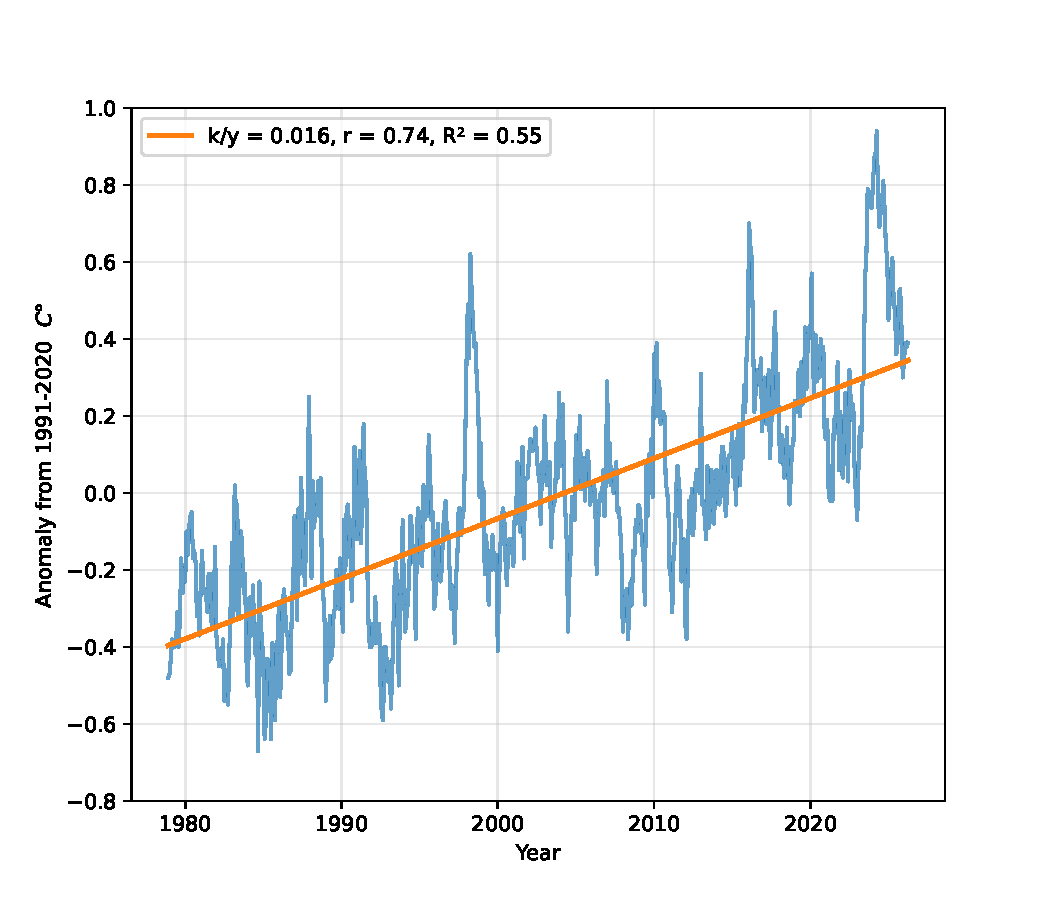
\includegraphics[scale=0.5]{img/uah-temp1.pdf}
    \caption{Long term trend, $0.16\degree$ per 10 years.}
    \label{fig:temp}
  \end{subfigure}%
  \begin{subfigure}{.5\paperwidth}
    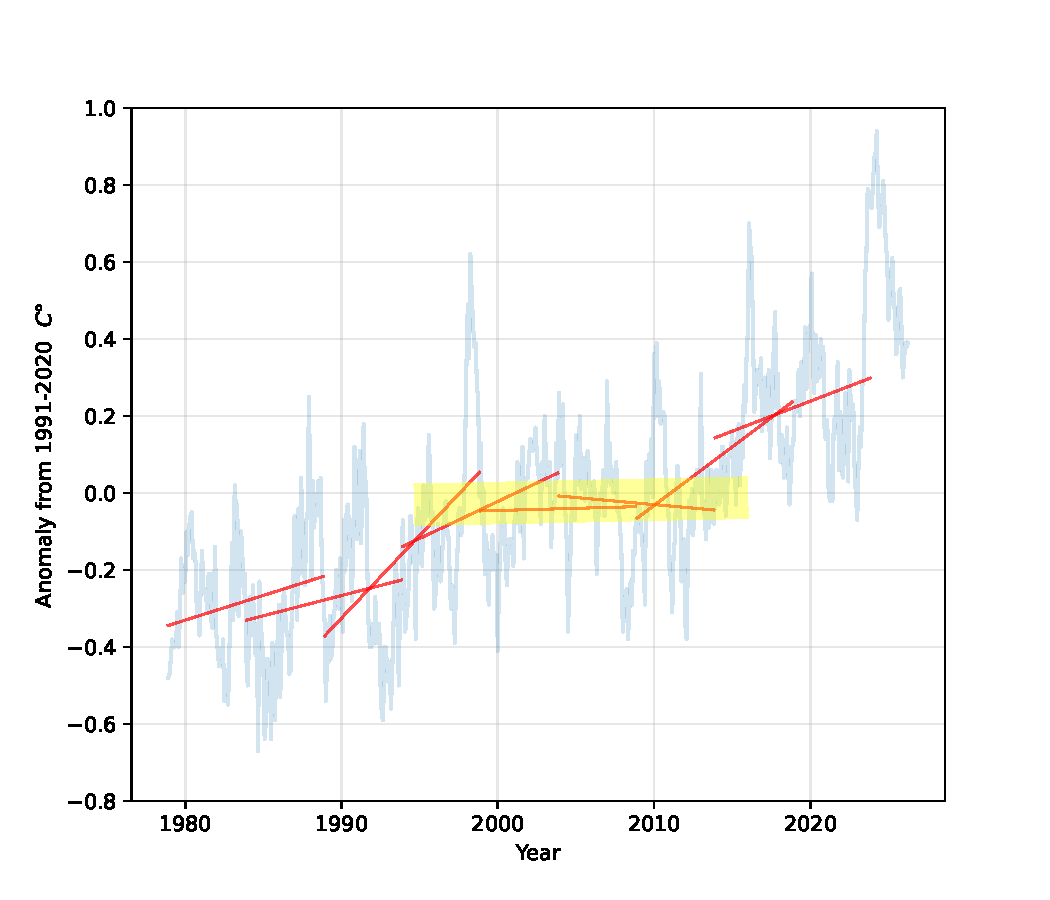
\includegraphics[scale=0.5]{img/uah-temp2.pdf}
    \caption{Short term trends (10 years).}
    \label{fig:trend}
  \end{subfigure}%
  \caption{Global temperature anomalies (1991-2020), UAH v6.0}
\end{figure}

The linear trend is of course what is the worry; even a modest
increase of $0.16\degree$ each decade will after some hundred years
add up. The question is if there is an underlying warming trend or if
what we see is only the result of random changes. The average global
temperature is of course not some random event; in the record we can
identify El Niño years and volcanic eruptions that have a large impact
on the global temperature. It is however interesting to see what the
temperature would look like if it was just a sequence of random
events.


\section*{Changes}

The global surface temperature is not a random variable; if it was it
would zig-zag its way around a mean value. If we look at the
temperature anomalies they have a mean of slightly below zero (it's the
anomaly from the 1990-2020 mean) and a standard deviation of $0.3$. If
we would generate a sequence from a random variable with a
natural distribution with these parameters, the temperature would most
of the time swing between $-0.3\degree$ and $0.3\degree$ - this is not
what we see.

The atmosphere, with a mass that can be compared to ten meters of
water covering the planet, has a memory and changes take
time. Changes from one month to the other are not arbitrary large,
they can, in extreme cases, be as much as three tenth of a degree,
but most changes are less than a tenth of a degree. The correlation
between temperature for two consecutive months is as
high as $0.9$ - the temperature next month does not vary much from
this month.

If however, we look at the increase from one month to the other, as
shown in Fig. \ref{fig:uah-diff}, we see that it looks almost like a
random variable. The distribution is close to a normal distribution
with mean zero and standard deviation of $0.12$. So even if the
temperature itself is not a random variable, the changes do look like
one.

\begin{figure}[t]
  \centering
  \hspace*{-3cm}
  \begin{subfigure}{.4\paperwidth}
    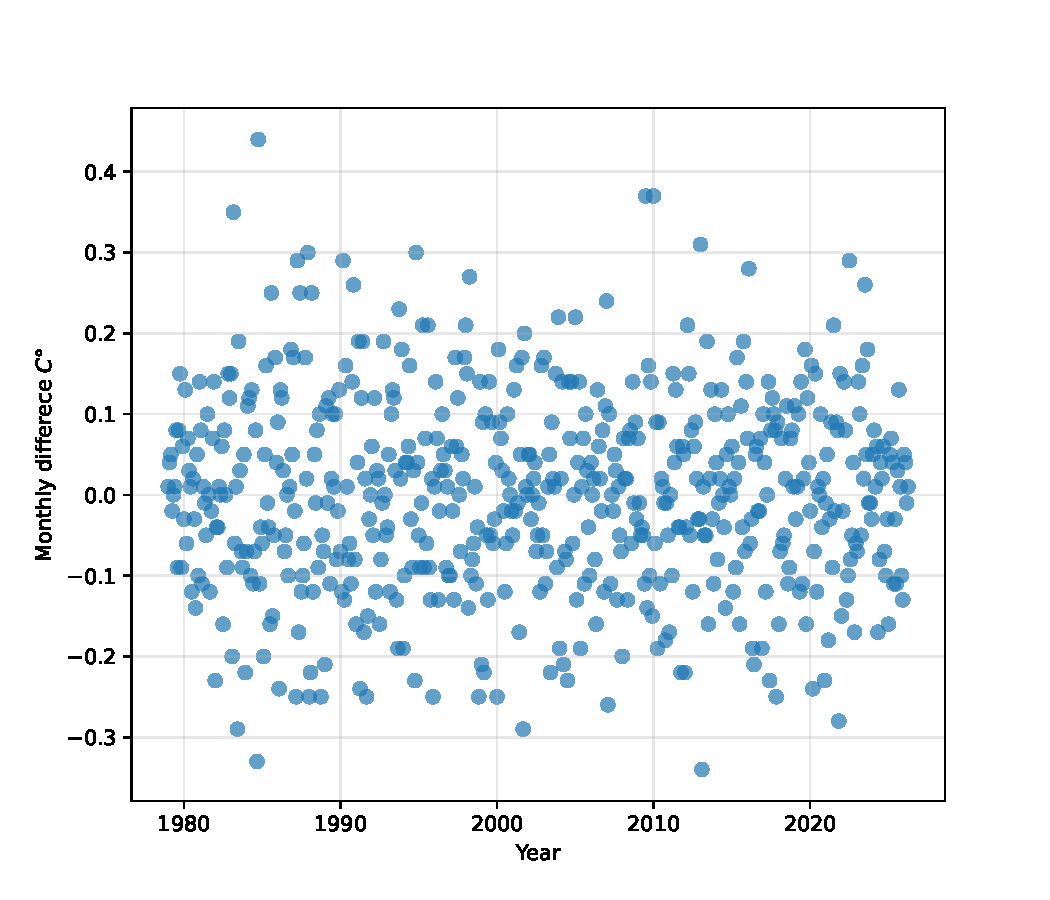
\includegraphics[scale=0.4]{img/uah-diff.pdf}
    \caption{Changes each month.}
  \end{subfigure}%
  \begin{subfigure}{.6\paperwidth}
    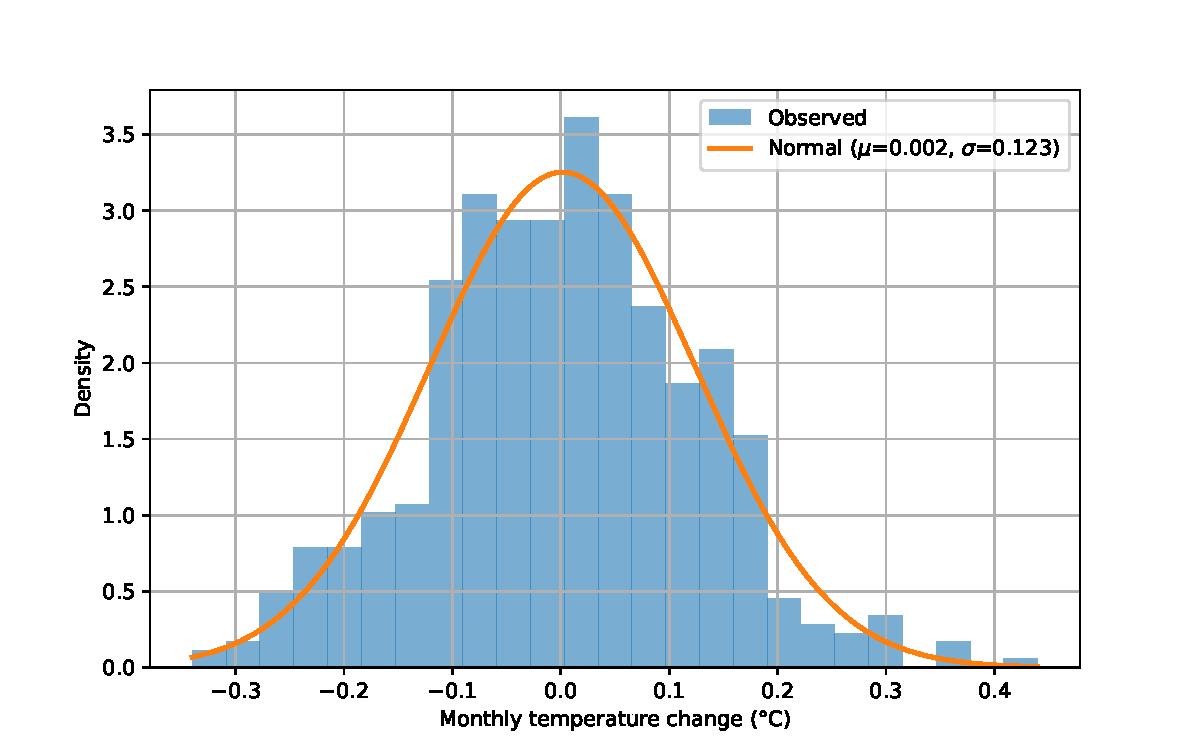
\includegraphics[scale=0.5]{img/uah-hist.pdf}
    \caption{Distribution of changes.}
  \end{subfigure}%  
  \caption{Monthly changes of temperature anomalies.}
  \label{fig:uah-diff}
\end{figure}

Could it be that the changes that we have seen over the last
45 years is just the result of random changes?

\section*{Random Walk}

If (it's not) the changes in temperature are drawn
from a random variable with a normal distribution of mean zero and
standard deviation of $0.12$, then we would not be surprised if the
temperature went up and down and after 45 years ended up plus or
minus some degrees. In Fig. \ref{fig:random} we see a collection of
such {\em random walks}, as clearly seen the
temperature would vary quite a lot; the actual temperature changes
now looks quite modest.


\begin{figure}[t]
  \centering
  \hspace*{-3cm}
  \begin{subfigure}{.5\paperwidth}
    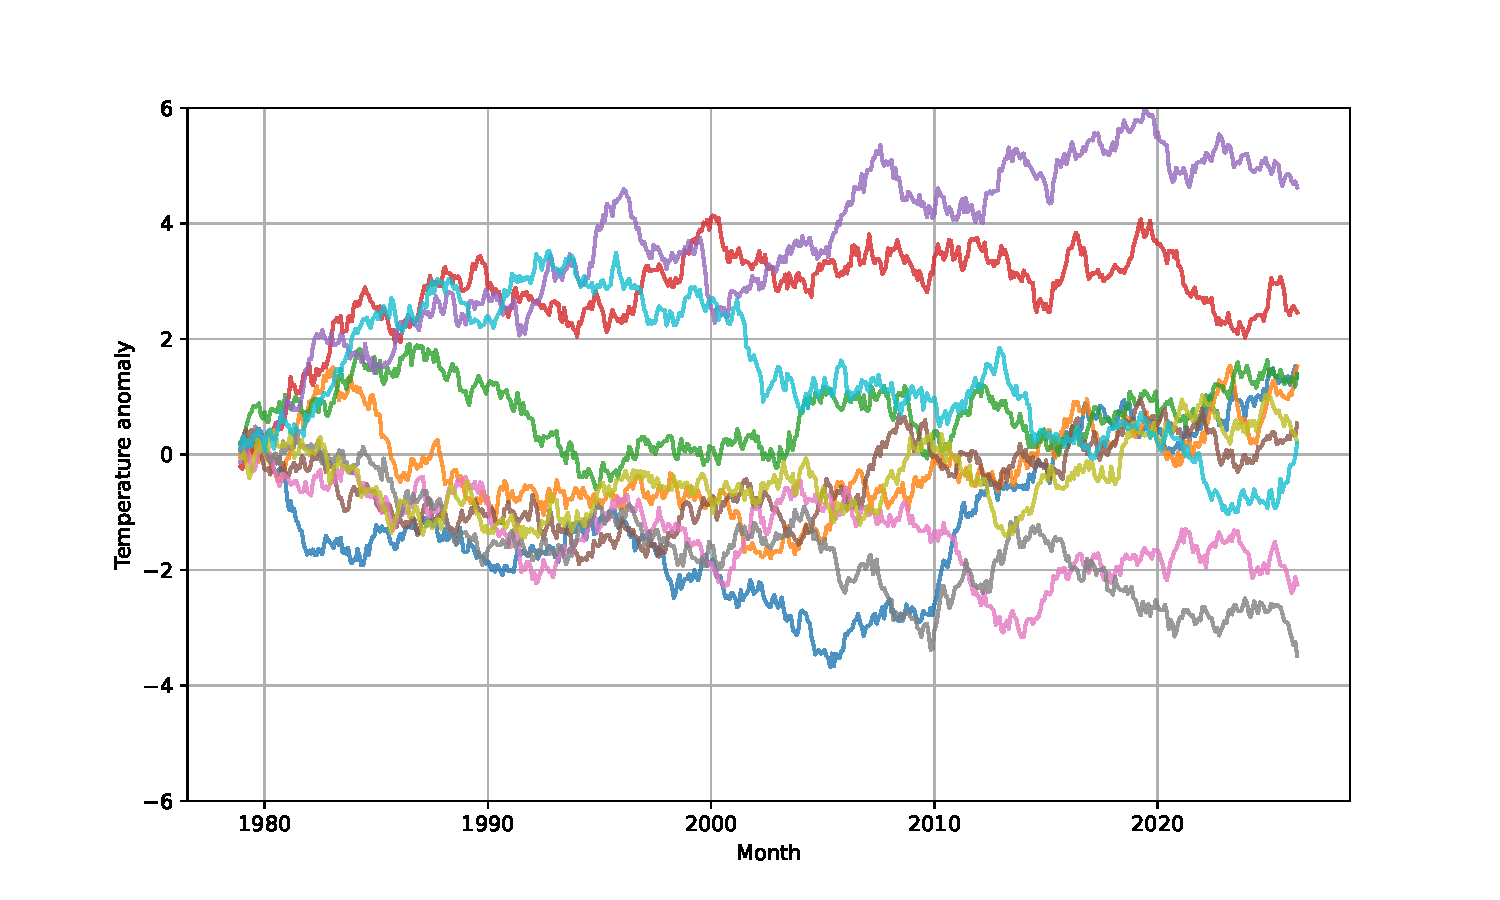
\includegraphics[scale=0.4]{img/random-walk.pdf}
    \caption{Random walks, all drawn from the same random variable.}
    \label{fig:random}
  \end{subfigure}%
  \begin{subfigure}{.5\paperwidth}
    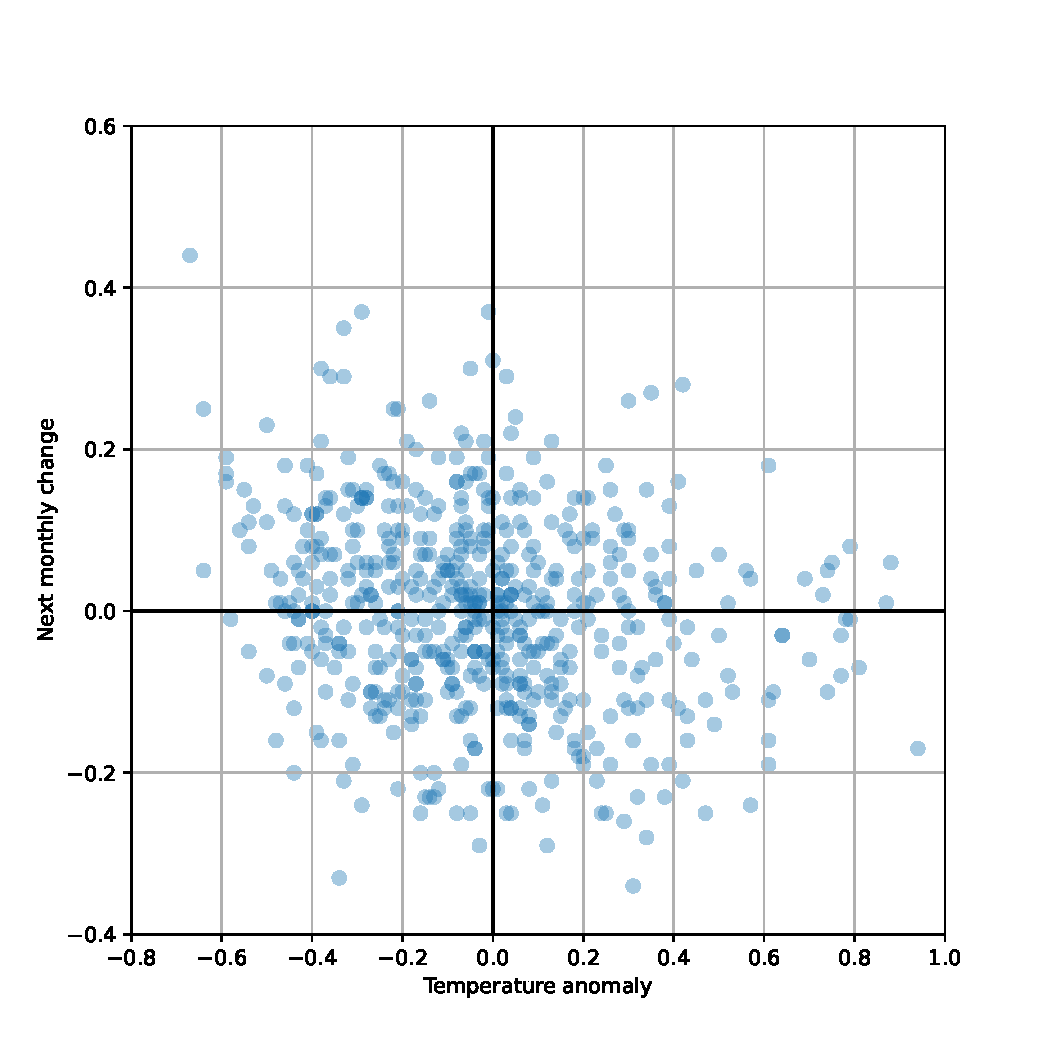
\includegraphics[scale=0.4]{img/corr-diff-temp.pdf}
    \caption{Correlation monthly changes and temperature.}
    \label{fig:changes}
  \end{subfigure}%  
  \caption{Monthly changes of temperature anomalies.}
\end{figure}

This is however not exactly what is happening. The changes that we see
one month actually depends on the temperature of the previous month. A
warm world will of course radiate more energy to space and radiation,
from a black body, is proportional to $T^4$ i.e. even a small change
in temperature will cause a big change in radiation. Now before we
panic we should realize that this is given absolute temperatures in
{\em Kelvin} and if it changes from say $285K$ to $285.5$ even a $T^4$
factor is not that big (less than one percent).

We can see this effect in a scatter plot of monthly changes vs
temperature as show in Fig. \ref{fig:changes}. The correlation is not
very strong (-0.21) but a linear regression has a gradient of
$-0.09$. If we want to model temperature change we should take this
into account.


\section*{Restoring force}

The temperature series that we are working with does, from a
statistical point of view, look like special form of random walk. It
does progress one step at the time but when the next step is taken it
is not drawn from a random variable but it takes the current
temperature into account. If the temperature is high it is more likely
to decrease the temperature rather than increasing it even more. This
tendency works both ways so a cold month is more likely to be followed
by a warmer month than an even colder month.

The model is called {\em stochastic process with a restoring
 force}. This, and more advanced models, are normally used to
describe series where there is an inherent lag but also a tendency to
return to {\em normal}.

If we model this behavior and start with the anomaly given by UAH in
1979, we get the plot shown in Fig. \ref{fig:model}. The measured
series, given by UAH, is nothing that stands out as abnormal. The four
generated series vary as much and also show ups and downs during the
period.

\begin{figure}[t]
  \centering
  \hspace*{-4cm}
  \begin{subfigure}{.5\paperwidth}
    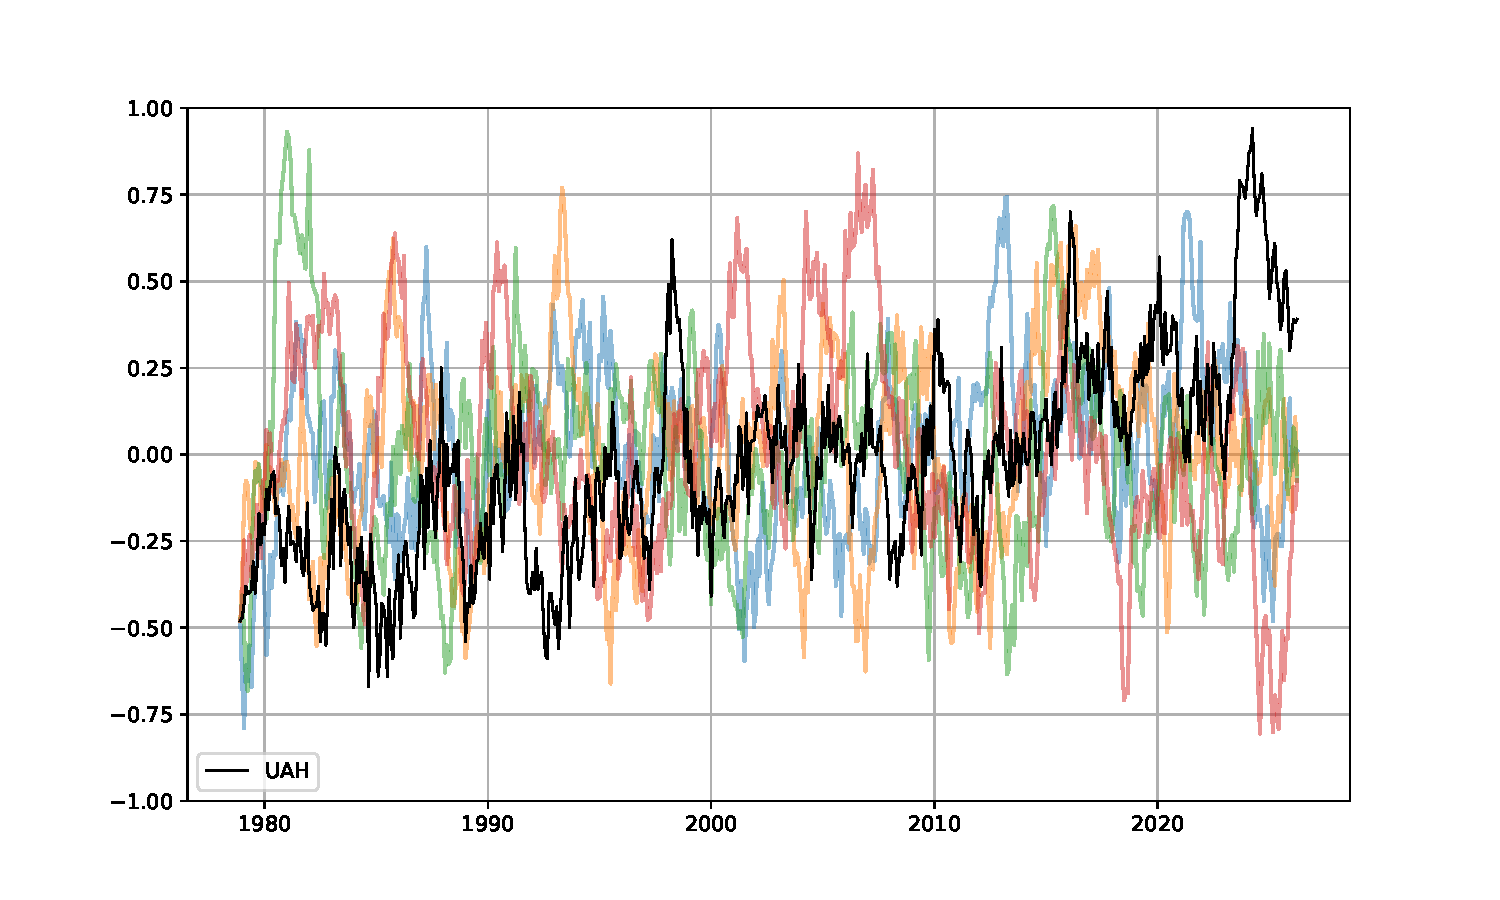
\includegraphics[scale=0.4]{img/model.pdf}
    \caption{Four generated series and UAH.}
    \label{fig:model}
  \end{subfigure}%
  \begin{subfigure}{.5\paperwidth}
    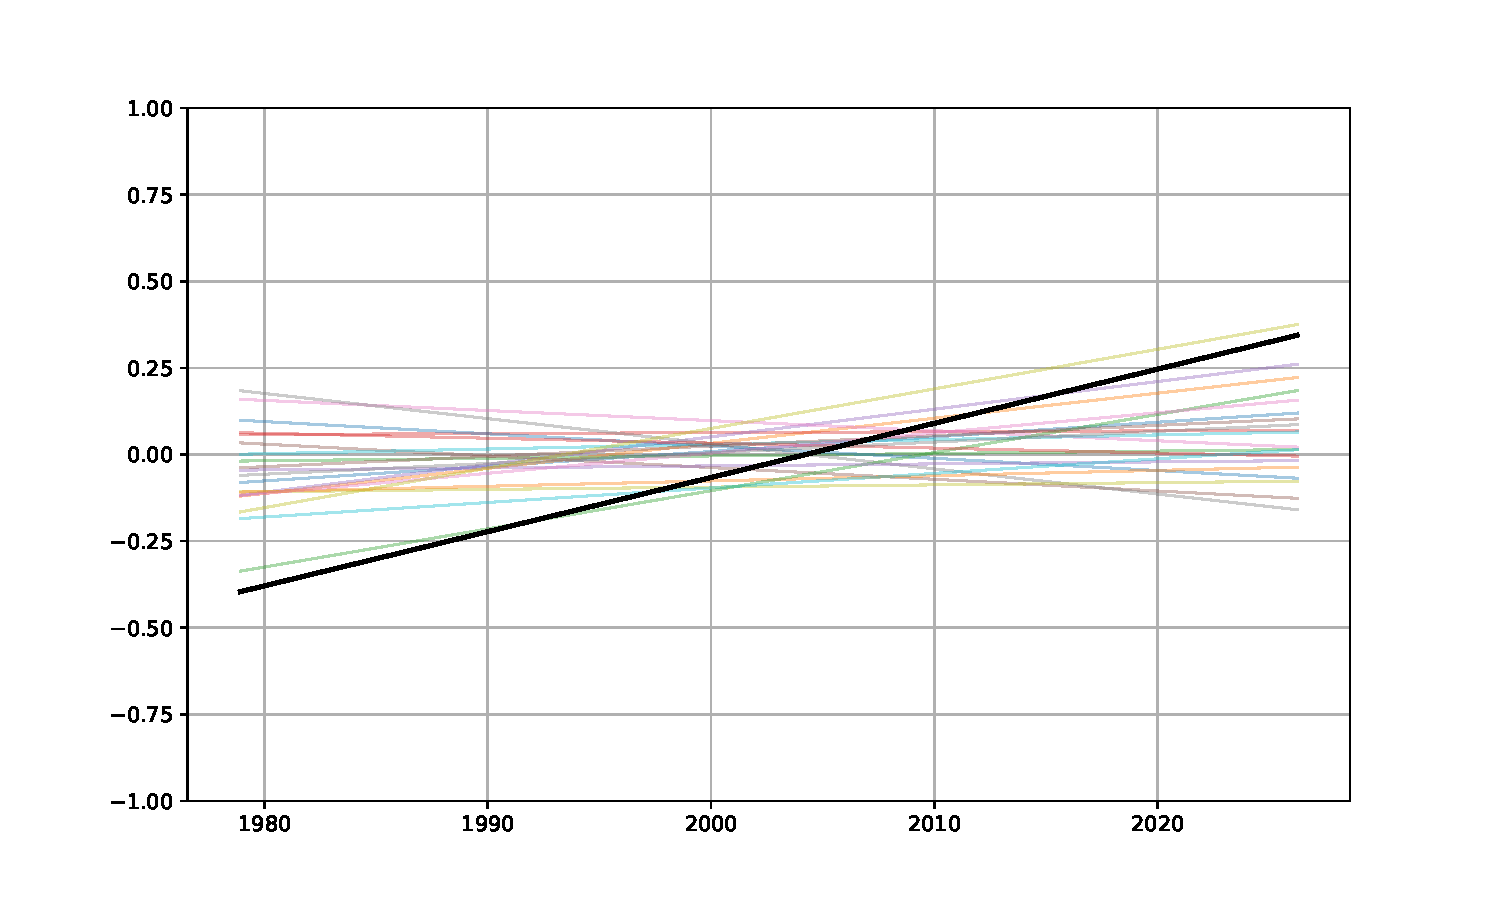
\includegraphics[scale=0.4]{img/model-trend.pdf}
    \caption{Linear trends of ten generated series and UAH.}
    \label{fig:trends}
  \end{subfigure}%  
  \caption{Model of temperature series given restoring force..}
\end{figure}

Although the UAH temperature series does not stand out as exceptional
it is actually a bit of an outlier. It does have a linear trend of
$0.16\degree$ per decade and this very high. In Fig. \ref{fig:trends}
we see the linear trends of twenty generated series and as can see they
show both negative and positive trends. The UAH series does however
stand out as an exception. 

If we study this further we can do a {\em Monte Carlo simulation} and
generate 10.000 series. We let the simulations start at the observed
temperature in 1979 and then collect the linear trends. The mean of
these trens is clse to zero and the standard deviation is close to
$0.04$ wich means that the observed trend is four standard deviations
from the mean. The observed temperature sequence would be an extreme
outlier if this would be the true distribution.

\section*{Mother Nature}

The global temperature is not a random process even though I think we
can say that it, from a statistical point of view, has traits of a
stochastic process with a returning force. The temperature records
that we do have for the last fifty years have a linear trend that is
larger than what one would expect from a monthly random process but then
the climate system is more complex.

Even though the temperature record can be modeled statistically as a
stochastic process it is of course a physical system where nothing
happens by chance (quantum effects besides). The temperature does not
suddenly rise without something happening. The things that do dictate
temperature changes are to a large extent so complicated and
unpredictable that we might as well treat them as random. That said,
there are of course many changes that we can attribute to natural
causes.

If we look at the diagram in Fig. \ref{fig:enso} we see the UAH
temperature anomaly series but also yellow sections where the so
called {\em Oceanic Niño Index} \cite{nino:oni} has been above a given
threshold for five consecutive months. The index is used to track the
{\em El Niño Southern Oscillation} that is a change in ocean currents
in the South Pacific. As, clearly seen this phenomena has an effect on
the global temperatures so from this perspective the changes in
temperature are not random.


\begin{figure}[t]
  \centering
  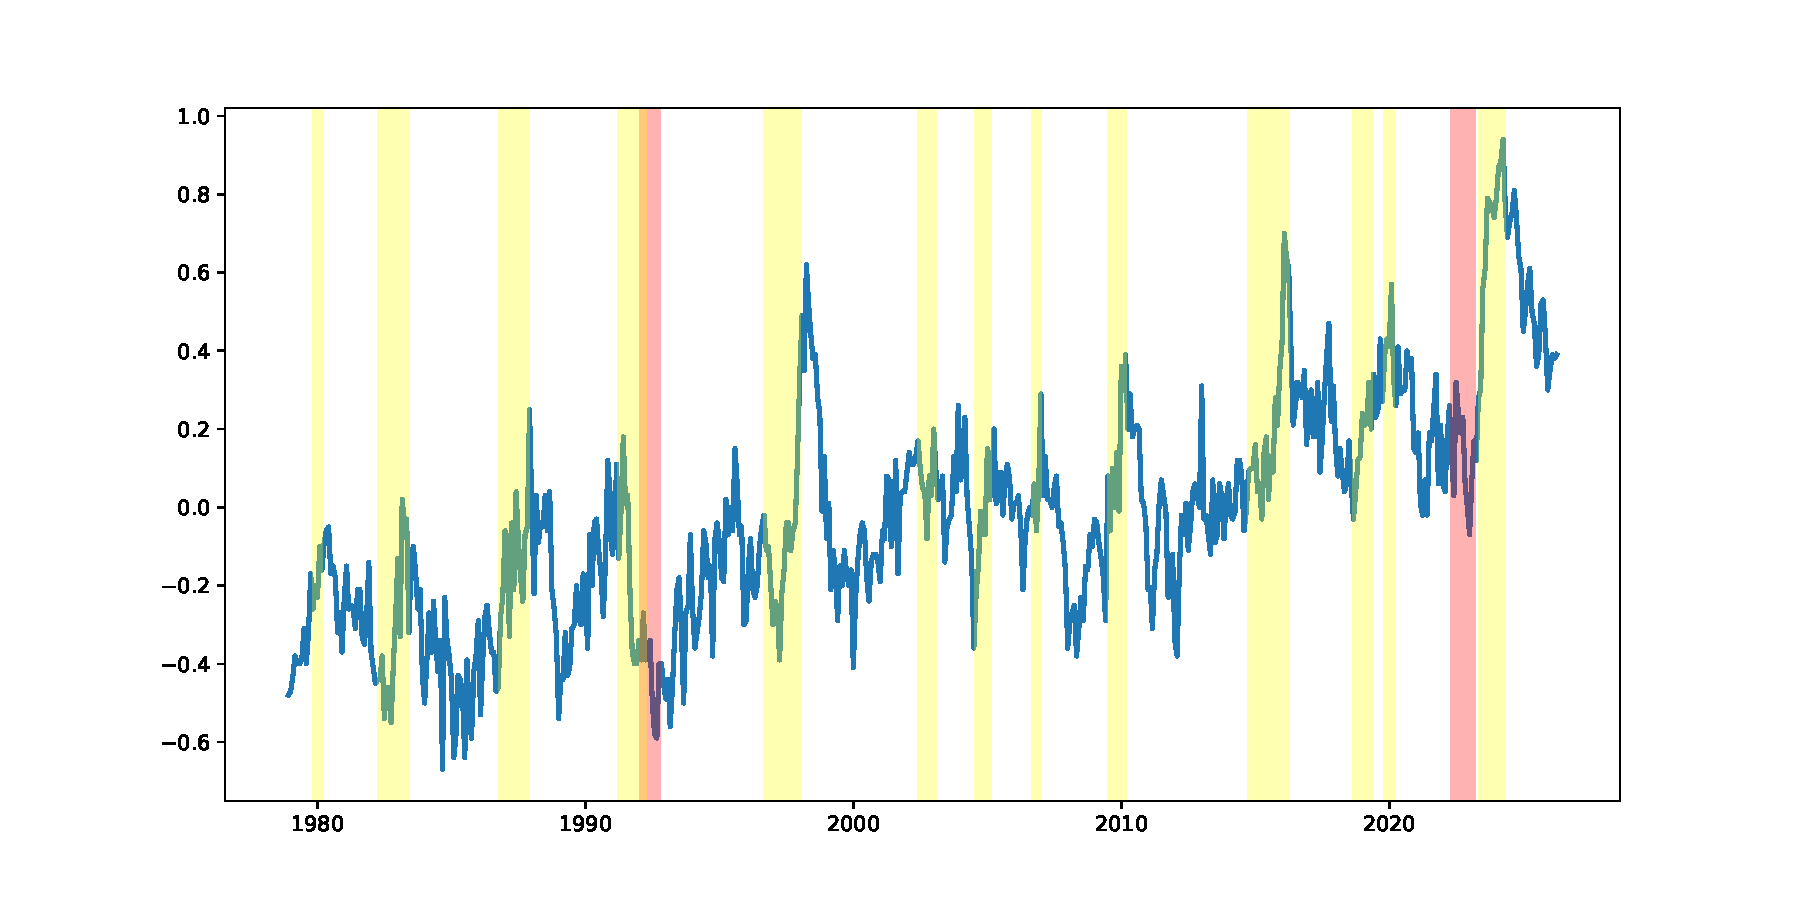
\includegraphics[scale=0.5]{img/enso.pdf}
  \caption{High Oceanic Niño Index (ONI) in yellow and large volcanic eruptions in red.}
  \label{fig:enso}
\end{figure}

In the graph we also have two major volcanic eruptions marked in
red. The Mount Pinatubo eruption in 1991 was the second-largest
eruption of the 20th century. Estimates are that the eruption caused
an initial $0.5\degree$ decrease in global temperatures and effects
that lasted for years \cite{parker:96}.

The eruption of Hunga Tonga–Hunga Ha'apai in 2022 might also have had
the opposite effect since the volcano was 150 m below the sea
surface. The explosion that followed threw so much water into the
stratosphere that it is likely that it contributed to the global
temperature increase for several years \cite{jenkins:22}.

Sea currents in the South Pacific and volcanic eruptions, are events
that last for several months to years. If we want to model the
temperature changes as a stocastic process we should take this into
account. We could group the temperature series into six-months
intervals and do a similar analysis as above. We then find that the
observed trend is still an outlier but not as extreme as before, less
than three standard deviations from the mean. If we look at the
simulated final temperatures then the observed final temperature is
well within two standard deviations of the distribution.

Before one digs deeper into these numbers one should of course ponder
if oceanic events such as El Niño are driving the global temperature
or, if they are driven by the global temperature. Shifts in ocean
currents could of course not add energy to the system, but it could
definitely change the distribution between ocean and atmosphere.


Since the oceans are a factor four hundred times larger than the
atmosphere it is not far fetched to think that even a small shift
could lead to the changes that we have seen. Since the oceans contain
vastly more thermal energy than the atmosphere, relatively small
changes in ocean-atmosphere heat exchange could potentially have a
substantial effect on atmospheric temperatures. Quantifying the
magnitude of this contribution is, however, beyond the scope of this
analysis.



\bibliographystyle{plain} % We choose the "plain" reference style
\bibliography{../bib/carbon} % Entries are in the refs.bib file

\end{document}
